\section{Graphical Models} 

  The concept of using latent variables to model some process will be used over and over again. We have seen simple examples of latent linear models, but what about nonlinear ones? It turns out that these can be seen as a specific instance of \textit{graphical models}. 

  When computing high-dimensional distributions, the parameters needed to encode this density scales badly. We can see that a general Gaussian mixture model in $\mathbb{R}^n$ with $k$ clusters requires $O(n^2 k)$ parameters. If we wanted to sample from a distribution of portraits, then the dimension $n$ would be the resolution of the image. For a $1024 \times 1024$ image, this requires $n = 3 \cdot 2^{20}$ dimensions, and modeling it with a GMM is hopeless. Fortunately, for complex distributions there is usually some dependencies (e.g. between neighboring pixels) that we can take advantage of. This is exactly what graphical models do. They factor complex distributions so that the scaling is much better. While there are graphical models that do not use latent variables, most interesting applications of graphical models require latent variables, and so we will focus on that. Additionally, we will introduce the EM algorithm, which will be used repeatedly and is particularly important in optimizing \textit{variational autoencoders} in deep learning. 

\subsection{Gaussian Mixture Models and EM Algorithm}

  Given a training set ${\mathbf{x}^{(i)}}_{i=1}^n$ (without the $y$-labels and so in the unsupervised setting), there are some cases where it may seem like we can fit multiple Gaussian distributions in the input space $\mathcal{X}$. For example, the points below seem like they can be fitted well with 3 Gaussians.

  \begin{figure}[H]
    \centering
    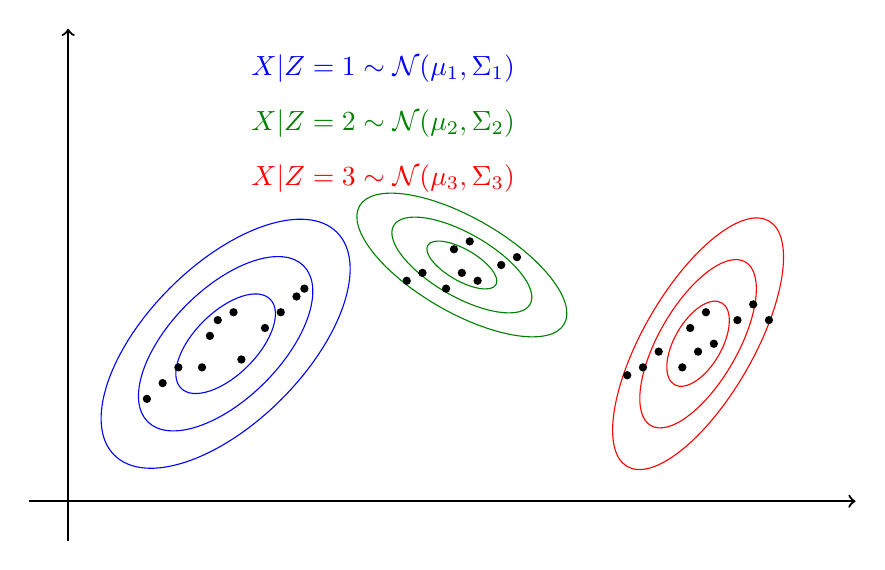
\begin{tikzpicture}
      % Draw axes
      \draw[black, ->, line width=0.8pt] (-0.5,0) -- (10,0);
      \draw[black, ->, line width=0.8pt] (0,-0.5) -- (0,6);
      
      % Equations at top
      \node[blue] at (4,5.5) {$X|Z=1 \sim \mathcal{N}(\mu_1, \Sigma_1)$};
      \node[green!50!black] at (4,4.8) {$X|Z=2 \sim \mathcal{N}(\mu_2, \Sigma_2)$};
      \node[red] at (4,4.1) {$X|Z=3 \sim \mathcal{N}(\mu_3, \Sigma_3)$};
      
      % First Gaussian (blue)
      \draw[blue, rotate around={45:(2,2)}] (2,2) ellipse (2 and 1);
      \draw[blue, rotate around={45:(2,2)}] (2,2) ellipse (1.4 and 0.7);
      \draw[blue, rotate around={45:(2,2)}] (2,2) ellipse (0.8 and 0.4);
      
      % Blue cluster points - more spread out
      \fill[black] (1.7,1.7) circle (1.5pt);
      \fill[black] (1.8,2.1) circle (1.5pt);
      \fill[black] (2.1,2.4) circle (1.5pt);
      \fill[black] (2.2,1.8) circle (1.5pt);
      \fill[black] (1.9,2.3) circle (1.5pt);
      \fill[black] (1.4,1.7) circle (1.5pt);
      \fill[black] (2.5,2.2) circle (1.5pt);
      \fill[black] (2.7,2.4) circle (1.5pt);
      \fill[black] (1.2,1.5) circle (1.5pt);
      \fill[black] (2.9,2.6) circle (1.5pt);
      \fill[black] (3.0,2.7) circle (1.5pt);
      \fill[black] (1.0,1.3) circle (1.5pt);
      
      % Second Gaussian (green)
      \draw[green!50!black, rotate around={-30:(5,3)}] (5,3) ellipse (1.5 and 0.6);
      \draw[green!50!black, rotate around={-30:(5,3)}] (5,3) ellipse (1 and 0.4);
      \draw[green!50!black, rotate around={-30:(5,3)}] (5,3) ellipse (0.5 and 0.2);
      
      % Green cluster points - more oval shaped
      \fill[black] (4.8,2.7) circle (1.5pt);
      \fill[black] (4.9,3.2) circle (1.5pt);
      \fill[black] (5.0,2.9) circle (1.5pt);
      \fill[black] (5.1,3.3) circle (1.5pt);
      \fill[black] (5.2,2.8) circle (1.5pt);
      \fill[black] (4.5,2.9) circle (1.5pt);
      \fill[black] (5.5,3.0) circle (1.5pt);
      \fill[black] (4.3,2.8) circle (1.5pt);
      \fill[black] (5.7,3.1) circle (1.5pt);
      
      % Third Gaussian (red)
      \draw[red, rotate around={60:(8,2)}] (8,2) ellipse (1.8 and 0.7);
      \draw[red, rotate around={60:(8,2)}] (8,2) ellipse (1.2 and 0.5);
      \draw[red, rotate around={60:(8,2)}] (8,2) ellipse (0.6 and 0.3);
      
      % Red cluster points - more spread out
      \fill[black] (7.8,1.7) circle (1.5pt);
      \fill[black] (7.9,2.2) circle (1.5pt);
      \fill[black] (8.0,1.9) circle (1.5pt);
      \fill[black] (8.1,2.4) circle (1.5pt);
      \fill[black] (8.2,2.0) circle (1.5pt);
      \fill[black] (7.5,1.9) circle (1.5pt);
      \fill[black] (8.5,2.3) circle (1.5pt);
      \fill[black] (7.3,1.7) circle (1.5pt);
      \fill[black] (8.7,2.5) circle (1.5pt);
      \fill[black] (8.9,2.3) circle (1.5pt);
      \fill[black] (7.1,1.6) circle (1.5pt);
    \end{tikzpicture}
    \caption{Example of data that can be fitted with 3 Gaussians}
  \end{figure}

  Therefore, we can construct a best-fit model as a composition of a multinomial distribution (to decide which one of the Gaussians $\mathbf{x}$ should follow) followed by a Gaussian. That is, to find the distribution of $\mathbf{x}$ and get the density function $p(\mathbf{x})$, we condition it on the random variable $Z$. More specifically, we let
  \begin{equation}
    Z \sim \text{Multinomial}(\boldsymbol{\phi}), \;\;\;\;\; \boldsymbol{\phi} = \begin{pmatrix} \phi_1 \ \phi_2 \ \ldots \ \phi_k \end{pmatrix} \text{ such that } \sum_{i=1}^k \phi_i = 1
  \end{equation}
  and define the conditional distributions as
  \begin{align*}
    \mathbf{X} \mid Z = 1 & \sim \mathcal{N}(\boldsymbol{\mu}_1, \boldsymbol{\Sigma}_1) \\
    \mathbf{X} \mid Z = 2 & \sim \mathcal{N}(\boldsymbol{\mu}_2, \boldsymbol{\Sigma}_2) \\
    \ldots & \sim \ldots \\
    \mathbf{X} \mid Z = j & \sim \mathcal{N}(\boldsymbol{\mu}_j, \boldsymbol{\Sigma}_j) \\
    \ldots & \sim \ldots \\
    \mathbf{X} \mid Z = k & \sim \mathcal{N}(\boldsymbol{\mu}_k, \boldsymbol{\Sigma}_k)
  \end{align*}
  Therefore, our model says that each $\mathbf{x}^{(i)}$ was generated by randomly choosing $z^{(i)}$ from ${1, \ldots, k}$ according to some multinomial, and then the $\mathbf{x}^{(i)}$ was drawn from one of the $k$ Gaussians depending on $z^{(i)}$. This model is called the \textbf{mixture of Gaussians model}. The parameters of our model are: 

  \begin{itemize}
    \item The vector $\boldsymbol{\phi} \in \mathbb{R}^k$ (which really has $k-1$ parameters) characterizing the multinomial distribution.
    \item The set of vectors $\boldsymbol{\mu}_1, \boldsymbol{\mu}_2, \ldots, \boldsymbol{\mu}_k$ representing the mean vectors of each multivariate Gaussian. For simplicity, we'll denote this set of vectors as $\bm{\mu}$.
    \item The set of symmetric, positive-definite matrices $\boldsymbol{\Sigma}_1, \boldsymbol{\Sigma}_2, \ldots, \boldsymbol{\Sigma}_k$ representing the covariance matrices of each multivariate Gaussian. For simplicity, we'll denote this set of matrices as $\bm{\Sigma}$.
  \end{itemize}

  We can write down the log-likelihood of the given data $\mathbf{x}^{(i)}$'s as a function of all the parameters above as:

  \begin{align*}
    l (\boldsymbol{\phi}, \bm{\mu}, \bm{\Sigma}) & = \sum_{i=1}^n \log, p\big( \mathbf{x}^{(i)} ;  \boldsymbol{\phi}, \bm{\mu}, \bm{\Sigma} \big) \\
    & = \sum_{i=1}^n \log \bigg( \sum_{j=1}^k  p\big( \mathbf{x}^{(i)} \mid z^{(i)} = j ; \bm{\mu}, \bm{\Sigma} \big) , p\big( z^{(i)} = j; \boldsymbol{\phi}\big) \bigg)
  \end{align*}

  This equation above tells us the (log-) likelihood of the data landing on the $\mathbf{x}^{(i)}$'s given that we have parameters $\boldsymbol{\phi}, \bm{\mu}, \bm{\Sigma}$. Note that since we only know that the \textit{final} value of the $i$th sample is $\mathbf{x}^{(i)}$ and not anything at all about which value $z^{(i)}$ the $i$th sample had, there is an extra unknown in this model. That is, we do not know which one of the $k$ Gaussians the $\mathbf{x}^{(i)}$ was generated from. These values $z^{(i)}$ are called the \textbf{hidden/latent variables}.

  If we did know the values of the hidden variables $z^{(i)}$ (i.e. if we knew which of the $k$ Gaussians each $\mathbf{x}^{(i)}$ was generated from), then our log likelihood function would be much more simple since now, our givens will be both $\mathbf{x}^{(i)}$ \textit{and} $z^{(i)}$. Therefore, we don't have to condition on the $z^{(i)}$ and can directly calculate the log of the probability of us having sample values $(z^{(1)}, \mathbf{x}^{(1)}), (z^{(2)}, \mathbf{x}^{(2)}), \ldots, (z^{(n)}, \mathbf{x}^{(n)})$.

  \begin{align*}
    l(\boldsymbol{\phi}, \bm{\mu}, \bm{\Sigma}) & = \sum_{i=1}^n \log , p\big( \mathbf{x}^{(i)}; \boldsymbol{\phi}, \bm{\mu} ,\bm{\Sigma}\big) \\
    & = \sum_{i=1}^n \log, p\big( \mathbf{x}^{(i)}, z^{(i)}; \boldsymbol{\phi}, \bm{\mu} ,\bm{\Sigma}\big) \\
    & = \sum_{i=1}^n \log, p\big( \mathbf{x}^{(i)} \mid z^{(i)}; \bm{\mu}, \bm{\Sigma}) \; p\big( z^{(i)}; \boldsymbol{\phi} \big)
  \end{align*}

  This model, with known $z^{(i)}$'s, is basically the GDA model, which is easy to calculate. That is, the maximum values of $\boldsymbol{\phi}, \bm{\mu}, \bm{\Sigma}$ are:

  \begin{align*}
    \phi_j & = \frac{1}{n} \sum_{i=1}^n \mathbbm{1}_{z^{(i)} = j} \\
    \boldsymbol{\mu}_j & = \frac{\sum_{i=1}^n \mathbbm{1}_{z^{(i)} = j} \mathbf{x}^{(i)}}{\sum_{i=1}^n \mathbbm{1}_{z^{(i)} = j}} \\
    \boldsymbol{\Sigma}_j & = \frac{1}{\sum_{i=1}^n \mathbbm{1}_{z^{(i)} = j}} \sum_{i=1}^n \mathbbm{1}_{z^{(i)}} \big( \mathbf{x}^{(i)} - \boldsymbol{\mu}_j \big),\big(\mathbf{x}^{(i)} - \boldsymbol{\mu}_j \big)^T
  \end{align*}

  for $j = 1, \ldots, d$. But since we do \textit{not} know the values of $z^{(i)}$, we first try to "guess" the values of the $z^{(i)}$'s and then update the parameters of our model assuming our guesses are correct. Let us clarify some notation:

  \begin{itemize}
    \item The distribution that we will iteratively reassign over and over again is $Z$, with density $p_Z (z)$ that maps $z \mapsto \phi_z$, where $\boldsymbol{\phi}$ is a vector that represents the density. The algorithm will initialize $p_Z$ and have it converge to the true multinomial density. Note that $Z$ in this context could represent the true multinomial distribution $Z$ or could represent the distributions iteratively produced by the algorithm that should converge onto the true $Z$ (usually the latter).

    \item The $k$ Gaussian distributions that we will iteratively reassign over and over again is $\mathcal{N}_1, \mathcal{N}_2, \ldots, \mathcal{N}k$, with densities $p_{\mathcal{N}1}(\mathbf{x}), \ldots, p_{\mathcal{N}k}(\mathbf{x})$ that maps $\mathbf{x} \mapsto p_{\mathcal{N}j}(\mathbf{x})$.

    \item The distribution of the entire random variable $\mathbf{X}$ will have density $p_X(\mathbf{x})$. Since we are iteratively reassigning the densities $p_Z$ and $p{\mathcal{N}_j}$, this joint distribution of $\mathbf{X}$ will also get modified.
  \end{itemize}

  \begin{definition}[EM Algorithm]
    The \textbf{Expectation-Maximization (EM) Algorithm} has the following steps:

    \begin{enumerate}
      \item We initialize our values of $\theta$, which can be chosen randomly or by \textbf{K-means initialization} (not explained here).
      \begin{itemize}
        \item We can randomly assign our values of $\mu_j$'s and the $\Sigma_j$'s in $\mathbb{R}^d$.
        \item We can randomly assign the density of our guess multinomial $p_Z(z)$, represented by vector
        \[\phi = \begin{pmatrix} \phi_1 \\ \vdots \\ \phi_k \end{pmatrix} \text{ with } \sum_{j=1}^k \phi_j = 1\]
        where $p_Z(z) \equiv \phi_z$ for $z = 1, \ldots, k$.
      \end{itemize}

      \item \textbf{(E Step)} Now that we have our prior guess of what $Z$ and its density function $p_Z$ is, we can calculate its posterior density function by taking one observed example $x^{(i)}$ and modifying $p_Z$ to $p_Z^{(i)}$. This superscript $(i)$ on the distribution $p_Z$ indicates that this is a posterior density created from observing $x^{(i)}$. (The motivation for this construction is explained more specifically in the next section involving Jensen's inequality.) Using Bayes' rule, we should calculate $n$ density functions
      \[p_Z^{(i)}(z) \equiv p_Z(z\,|\,x^{(i)}; \phi, \mathbf{\mu}, \mathbf{\Sigma}) \text{ for } i = 1, \ldots, n\]
      For easier notation, we let $\phi^{(i)}$ be the vector representation of the density $p_Z^{(i)}$. That is,
      \[\phi^{(i)} = \begin{pmatrix} \phi_1^{(i)} \\ \vdots \\ \phi_k^{(i)} \end{pmatrix} \text{ with } \sum_{j=1}^k \phi_j^{(i)} = 1\]
      where $p_Z^{(i)}(z) \equiv \phi^{(i)}_z$ for $z = 1, \ldots, k$ and $0$ otherwise. Then, we can calculate $\phi^{(i)}$ (and therefore $p_Z^{(i)}$) component-wise by calculating each $\phi_j^{(i)}$ (which is the probability of a point being in the $j$th cluster, given that we observe example $x^{(i)}$):
      \begin{align*}
          \phi_j^{(i)} &= p_Z^{(i)}\big(z = j;\, \phi, \mathbf{\mu}, \mathbf{\Sigma}\big) \\
          &= p_Z\big(z = j\,|\,x^{(i)};\,\phi, \mathbf{\mu}, \mathbf{\Sigma}\big) \\
          &= \frac{p_{\mathcal{N}_j}\big(x^{(i)}\,|\,z^{(i)} = j;\,\mathbf{\mu}, \mathbf{\Sigma}\big) \; p_Z\big(z^{(i)} = j;\,\phi\big)}{p_X\big(x^{(i)};\,\phi, \mathbf{\mu}, \mathbf{\Sigma}\big)} \\
          &= \frac{p_{\mathcal{N}_j}\big(x^{(i)}\,|\,z^{(i)} = j;\,\mathbf{\mu}, \mathbf{\Sigma}\big) \; p_Z\big(z^{(i)} = j;\,\phi\big)}{\sum_{l=1}^k p_{\mathcal{N}_j}\big(x^{(i)}\,|\,z^{(i)} = l;\,\mathbf{\mu}, \mathbf{\Sigma}\big)\; p_Z\big(z^{(i)} = l;\,\phi\big)}
      \end{align*}
      Note that we have everything we need to calculate the posterior probability distribution $p_Z^{(i)}(z)$ of a point being in any cluster.
      \begin{itemize}
          \item $p_{\mathcal{N}_j}(x^{(i)}\,|\,z^{(i)} = j)$ represents the conditional Gaussian density, which is completely defined because the parameters $\mu_j, \Sigma_j$ are already defined in initialization.
          \item $p_Z(z^{(i)} = j; \phi)$ is really just the probability $\phi_j$ that a given point is in the $j$th cluster, which we've also defined in initialization.
          \item $p_X(x^{(i)})$ represents the distribution of the entire random variable $X$ of the entire training set. Knowing the first two and taking the sum gives this density function $p_X$.
      \end{itemize}
      Therefore, we should end up with $n$ different $k$-vectors $\phi^{(1)}, \phi^{(2)}, \ldots, \phi^{(n)}$, each representing our best guess of what multinomial density $p_Z^{(i)}$ each $x^{(i)}$ had followed in order to be at the given points.


      \begin{figure}[H]
        \centering
        \begin{subfigure}[b]{0.48\textwidth}
          \centering
          \begin{tikzpicture}[scale=1.]
            \draw[->] (-0.5,0) -- (5,0);
            \draw[->] (0,-0.5) -- (0,3.5);
            
            % Points and labels
            \fill[red] (1,1) circle (3pt);
            \fill[red] (1.5,0.8) circle (3pt);
            \fill[red] (2,1.5) circle (3pt);
            \node[red] at (3,1.5) {$\phi_1=\frac{3}{6}$};
            
            \fill[blue] (3,2.5) circle (3pt);
            \fill[blue] (3.2,2) circle (3pt);
            \node[blue] at (4,2.5) {$\phi_2=\frac{2}{6}$};
            
            \fill[green!50!black] (4,1) circle (3pt);
            \node[green!50!black] at (4.5,1) {$\phi_3=\frac{1}{6}$};
          \end{tikzpicture}
          \caption{Hard label assignments.}
          \label{fig:hard-guesses}
        \end{subfigure}
        \hfill 
        \begin{subfigure}[b]{0.48\textwidth}
          \centering
          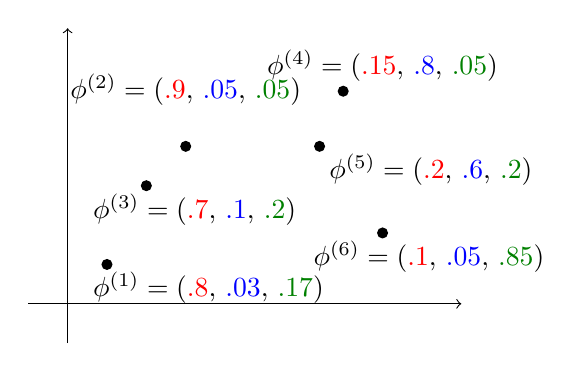
\begin{tikzpicture}[scale=1]
            \draw[->] (-0.5,0) -- (5,0);
            \draw[->] (0,-0.5) -- (0,3.5);
            
            % Points and colored vectors
            \fill (0.5,0.5) circle (2pt);
            \node[right] at (0.2,0.2) {$\phi^{(1)} = ($\textcolor{red}{.8}, \textcolor{blue}{.03}, \textcolor{green!50!black}{.17}$)$};
            
            \fill (1.5,2) circle (2pt);
            \node[above] at (1.5,2.4) {$\phi^{(2)} = ($\textcolor{red}{.9}, \textcolor{blue}{.05}, \textcolor{green!50!black}{.05}$)$};
            
            \fill (1,1.5) circle (2pt);
            \node[right] at (0.2,1.2) {$\phi^{(3)} = ($\textcolor{red}{.7}, \textcolor{blue}{.1}, \textcolor{green!50!black}{.2}$)$};
            
            \fill (3.5,2.7) circle (2pt);
            \node[above] at (4,2.7) {$\phi^{(4)} = ($\textcolor{red}{.15}, \textcolor{blue}{.8}, \textcolor{green!50!black}{.05}$)$};
            
            \fill (3.2,2) circle (2pt);
            \node[right] at (3.2,1.7) {$\phi^{(5)} = ($\textcolor{red}{.2}, \textcolor{blue}{.6}, \textcolor{green!50!black}{.2}$)$};
            
            \fill (4,0.9) circle (2pt);
            \node[right] at (3,0.6) {$\phi^{(6)} = ($\textcolor{red}{.1}, \textcolor{blue}{.05}, \textcolor{green!50!black}{.85}$)$};
          \end{tikzpicture}
          \caption{Soft probability assignments.}
          \label{fig:soft-guesses}
        \end{subfigure}
        \caption{Let us elaborate further on the intuition of this step. In the normal GDA with given values of $z^{(i)}$, we have $\phi_j = \frac{1}{n} \sum_{i=1}^n 1\{z^{(i)} = j\} = \frac{1}{n}\big(\text{Number of Samples in }j\text{th Gaussian}\big)$, which is a sum of "hard" guesses, meaning that each $x^{(i)}$ is undoubtedly in cluster $j$ or not, and so to find out our best guess for the true vector $\phi$, all we have to do is find out the proportion of all examples in each of the $k$ groups and we're done (without needing to iterate). However, in our EM model, we do not know the $z^{(i)}$'s, and so the best we can do is give the \textit{probability} $\phi^{(i)}_j$ that $x^{(i)}$ is in cluster $j$. So for each point $x^{(i)}$, the model has changed from it being undoubtedly in group $z^{(i)} = j$ to it having a probability of being in $\phi^{(i)}_j$ for $j = 1, \ldots, k$.}
        \label{fig:guesses-comparison}
      \end{figure}

      \item \textbf{(M Step)} With these $n$ separate posterior estimates of $Z$ for each observation $x^{(i)}$, we can simply average all of them and say that our best estimate of $\phi$ is
      \[\phi = \frac{1}{n} \sum_{i=1}^n \phi^{(i)}\]
      We can interpret the vectors $\phi^{(i)}$ as tuples where $\phi^{(i)}_j$ describes the expected "portion" of each sample $x^{(i)}$ to be in group $j$. So, we are adding up all the "portions" of the points that are expected to be in cluster $j$ to get $\phi_j = \sum_{i=1}^n \phi_j^{(i)}$.

      Now, given the $j$th Gaussian cluster, we would like to compute its mean $\mu_j$. Since each $x^{(i)}$ has probability $\phi^{(i)}_j$ of being in cluster $j$, we can weigh each of the $n$ points by $\phi^{(i)}_j$ (which determines how "relevant" $x^{(i)}$ is to cluster $j$) and average these (already weighted) points to get our "best-guess" of the mean $\mu_j$.
      \[\mu_j = \frac{\sum_{i=1}^n \phi^{(i)}_j x^{(i)}}{\sum_{i=1}^n \phi_j^{(i)}}\]

      \begin{figure}[H]
        \centering 
        \includegraphics[scale=0.27]{img/weighted_means.jpg}
        \caption{} 
        \label{fig:weighted_means}
      \end{figure}

      With this logic of weighted points, we finally update the covariance matrices $\Sigma_j$ as below:
      \[\Sigma_j = \frac{1}{\sum_{i=1}^n \phi_j^{(i)}} \sum_{i=1}^n \phi^{(i)}_j \,\big(x^{(i)} - \mu_j\big)\big(x^{(i)} - \mu_j\big)^T\]

      \item Now, we have new values of $\phi, \mu_1, \ldots, \mu_k, \Sigma_1, \ldots, \Sigma_k$ that we can work with. With these new values, repeat steps 2 and 3 until convergence.
    \end{enumerate}
  \end{definition}

  In summary, this entire algorithm results from modifying the "hard" data of each point $x^{(i)}$ being undoubtedly in one cluster to a model containing points $x^{(i)}$ that have been "smeared" around different clusters, with a probability $\phi_j^{(i)}$ being in cluster $j$. 

  \begin{definition}[Mixture of Gaussians Algorithm: Summary]
    Given a training set $\{x^{(i)}\}_{i=1}^n \in \mathbb{R}^d$, let us assume that the random variable $X$ that these examples follow can be modeled by specifying a joint distribution of a multinomial and Gaussians. 
    That is, it follows a Gaussian mixture model (GMM) of $k$ Gaussian clusters. Let
    \begin{itemize}
      \item $Z$ be the multinomial distribution representing which Gaussian cluster each example $x$ falls in, with density represented by vector $\phi \in \mathbb{R}^k$ so that $\mathbb{P}(Z = j) \equiv \phi_j$.
      \item The set of conditional distributions 
        \[X\,|\,Z = j \sim \mathcal{N}(\mu_j, \Sigma_j) \text{ for } j = 1, 2, \ldots, k\]
      are multivariate Gaussian, with mean vectors $\mu_1, \ldots, \mu_k$ and covariance matrices $\Sigma_1, \ldots, \Sigma_k$. 
    \end{itemize}
    Let all the parameters be denoted as $\theta$. Then, the EM algorithm is as such: 
    \begin{enumerate}
      \item Initialize the multinomial vector $\phi$, the $\mu_j$'s, and the $\Sigma_j$'s.
      \item \textbf{(E Step)} Calculate the $n$ vectors
        \[\phi^{(i)} = \begin{pmatrix} \phi_1^{(i)} \\ \vdots \\ \phi_k^{(i)} \end{pmatrix} \text{ for all } i = 1, \ldots, n\]
      that represent the posterior distribution of $Z$ given observed $x^{(i)}$ by computing 
        \begin{align*} 
          \phi_j^{(i)} & = p_Z^{(i)} \big(z = j;\, \phi, \mathbf{\mu}, \mathbf{\Sigma} \big) \\
          & = p_Z \big(z = j\,|\, x^{(i)}; \, \phi, \mathbf{\mu}, \mathbf{\Sigma} \big) \\
          & = \frac{p_{\mathcal{N}_j} \big(x^{(i)}\,|\,z^{(i)} = j; \, \mathbf{\mu}, \mathbf{\Sigma}\big) \; p_Z \big(z^{(i)} = j;\, \phi \big)}{p_X \big(x^{(i)};\, \phi, \mathbf{\mu}, \mathbf{\Sigma}\big)} \\
          & = \frac{p_{\mathcal{N}_j} \big(x^{(i)}\,|\,z^{(i)} = j; \, \mathbf{\mu}, \mathbf{\Sigma}\big) \; p_Z \big(z^{(i)} = j;\, \phi \big)}{\sum_{l=1}^k p_{\mathcal{N}_j} \big( x^{(i)}\,|\, z^{(i)} = l;\, \mathbf{\mu}, \mathbf{\Sigma} \big)\; p_Z \big(z^{(i)} = l; \,\phi\big)}
        \end{align*}
      \item \textbf{(M Step)} Reassign the value of $\theta$ as 
        \begin{align*} 
          \phi & = \frac{1}{n} \sum_{i=1}^n \phi^{(i)} \\
          \mu_j & = \frac{\sum_{i=1}^n \phi_j^{(i)} x^{(i)}}{\sum_{i=1}^n w_j^{(i)}} \text{ for } j = 1, \ldots, n \\
          \Sigma_j & = \frac{1}{\sum_{i=1}^n \phi_j^{(i)}} \sum_{i=1}^n \phi^{(i)}_j \, \big(x^{(i)} - \mu_j \big) \big(x^{(i)} - \mu_j\big)^T \text{ for } j = 1, \ldots, n 
        \end{align*}
      \item Repeat steps 2 and 3 until convergence.
    \end{enumerate}
  \end{definition}

\subsection{Bayesian Networks (Directed Graphical Models)} 

  Note that the whole purpose of directed graphical models is to model some sort of \textit{causal} relationship between two random variables. Note that while this is successful in practice, there is really no way to know for sure about any causality. 

  \begin{definition}[Bayesian Network]  
    A \textbf{Bayesian network}, also known as a \textbf{directed probability model}, is a directed acyclic graph of $M$ nodes representing a joint probability distribution of $M$ scalar random variables. An edge pointing $A \rightarrow B$ means that the $B$ is conditionally dependent on $A$, and that there is a very clear casual relationship coming from $A$ to $B$. The \textbf{parents} of a node $x_i$ is denoted $\mathrm{pa}_i$, and the entire joint distribution can be broken up as such: 
    \begin{equation}
      p(\mathbf{x}) = \prod_{m=1}^M p(x_m \mid x_{\mathrm{pa}_m})
    \end{equation}
    which is unique due to it being a DAG. Not only is a Bayesian network easy to parameterize. We can also sample from the joint distribution by sequentially sampling starting from the parents to the final children, and discarding the ones (marginalizing) that we don't wish to sample. This is known as \textbf{ancestral sampling}. 

    \begin{figure}[H]
      \centering 
      \begin{tikzpicture}[node distance=2cm]
        \node [node_style] (x1) at (0,0) {$x_1$};
        \node [node_style] (x2) at (-1,-1.5) {$x_2$};
        \node [node_style] (x3) at (1,-1.5) {$x_3$};
        \node [node_style] (x4) at (0,-3) {$x_4$};
        
        \draw [edge_style] (x1) -- (x2);
        \draw [edge_style] (x1) -- (x3);
        \draw [edge_style] (x2) -- (x4);
        \draw [edge_style] (x3) -- (x4);
        
        \node [above=0.2cm of x1] {Root Node};
        \node [below=0.2cm of x4] {Child Node};
      \end{tikzpicture}
      \caption{} 
      \label{fig:bayesian_network}
    \end{figure}
  \end{definition}

  This following example cleared up any confusion when I learned Bayesian networks for the first time. 

  \begin{example}[Relay Race]
    Consider a $4\times100$m relay race where the final race time depends on multiple factors. We can model this as a Bayesian network where the total race time $T$ depends on:
    \begin{itemize}
      \item Individual runner capabilities ($R_1$, $R_2$, $R_3$, $R_4$)
      \item Handoff success between runners ($H_1$, $H_2$, $H_3$)
      \item Individual leg performances ($P_1$, $P_2$, $P_3$, $P_4$)
    \end{itemize}

    The joint probability distribution factorizes as:
    \begin{align*}
      & p(T, R_1, R_2, R_3, R_4, H_1, H_2, H_3, P_1, P_2, P_3, P_4) = \\
      & p(T|P_1,P_2,P_3,P_4) \prod_{i=1}^4 p(R_i) \prod_{i=1}^3 p(H_i|R_i,R_{i+1}) \prod_{i=1}^4 p(P_i|R_i,H_{i-1})
    \end{align*}

    \noindent where $H_0$ is undefined for $P_1$, and each runner's performance depends on their capability and the success of the previous handoff (except for the first runner). This network captures both the individual contributions and the critical dependencies between runners during baton exchanges.

    \begin{figure}[H]
      \centering 
      \begin{tikzpicture}[node distance=2cm]
        % Runner nodes
        \node[runner_node] (r1) at (0,0) {$R_1$};
        \node[runner_node] (r2) at (2,0) {$R_2$};
        \node[runner_node] (r3) at (4,0) {$R_3$};
        \node[runner_node] (r4) at (6,0) {$R_4$};
        
        % Handoff nodes
        \node[factor_node] (h1) at (1,-1.5) {$H_1$};
        \node[factor_node] (h2) at (3,-1.5) {$H_2$};
        \node[factor_node] (h3) at (5,-1.5) {$H_3$};
        
        % Performance nodes
        \node[factor_node] (p1) at (0,-3) {$P_1$};
        \node[factor_node] (p2) at (2,-3) {$P_2$};
        \node[factor_node] (p3) at (4,-3) {$P_3$};
        \node[factor_node] (p4) at (6,-3) {$P_4$};
        
        % Final outcome
        \node[outcome_node] (result) at (3,-4.5) {$T$};
        
        % Draw edges
        % Runner to handoff connections
        \draw[edge_style] (r1) -- (h1);
        \draw[edge_style] (r2) -- (h1);
        \draw[edge_style] (r2) -- (h2);
        \draw[edge_style] (r3) -- (h2);
        \draw[edge_style] (r3) -- (h3);
        \draw[edge_style] (r4) -- (h3);
        
        % Handoff to performance connections
        \draw[edge_style] (h1) -- (p2);
        \draw[edge_style] (h2) -- (p3);
        \draw[edge_style] (h3) -- (p4);
        
        % Runner to their performance connections
        \draw[edge_style] (r1) -- (p1);
        \draw[edge_style] (r2) -- (p2);
        \draw[edge_style] (r3) -- (p3);
        \draw[edge_style] (r4) -- (p4);
        
        % Performance to final outcome connections
        \draw[edge_style] (p1) -- (result);
        \draw[edge_style] (p2) -- (result);
        \draw[edge_style] (p3) -- (result);
        \draw[edge_style] (p4) -- (result);
      \end{tikzpicture}
      \caption{Bayesian Network for a 4x100m Relay Race. The graphical representation is much more compact and intuitive than simply writing out all the products. }
      \label{fig:relay_race}
    \end{figure}
  \end{example} 

  Bayesian modelling with hierarchical priors. 

  \begin{example}[Multinomial]
    We first provide some motivation from a computational complexity perspective. Given a joint distribution of 2 random variables $\mathbf{x}_1, \mathbf{x}_2$, say which are multinomial with $K$ classes, their joint distribution $p(\mathbf{x}_1, \mathbf{x}_2)$ is captured by $K^2 - 1$ parameters. For a general $M$ random variables, then we have to keep a total of $K^M - 1$ parameters, and this increases exponentially. By building a directed graph with say $r$ maximum number of variables appearing on either side of the conditioning bar in a single probability distribution, then the computational complexity scales as $O(K^r)$, which may save a lot of time if $r << M$. 
  \end{example}

  Extending upon this example, we can see that we want to balance two things: 
  \begin{enumerate} 
    \item Fully conncted graphs have completely general distributions and have $O(K^M -1)$ number of parameters (too complex). 
    \item If there are no links, the joint distribution fully factorizes into the product of its marginals and has $M(K-1)$ parameters (too simple) . 
  \end{enumerate}
  Graphs that have an intermediate level of connectivity allow for more general distributions compared to the fully factorized one, while requiring fewer parameters than the general joint distribution. One model that balances this out is the hidden markov model. 

  \begin{example}[Chain Graph]
    Consider an $M$-node Markov chain. The marginal distribution $p(\mathbf{x}_1)$ requires $K-1$ parameters, and the remaining conditional distributions $p(\mathbf{x}_i \mid \mathbf{x}_{i-1})$ requires $K(K-1)$ parameters. Therefore, the total number of parameters is 
    \begin{equation}
      K-1 + (M-1) (K-1) K \in O(M K^2)
    \end{equation}
    which scales relatively well, and we have 
    \begin{equation}
      p(\{\mathbf{x}_m\}) = p (\mathbf{x}_1) \prod_{m=2}^M p(\mathbf{x}_m \mid \mathbf{x}_{m-1})
    \end{equation}
    \begin{center}
      TBD
    \end{center}
    We can turn this same graph into a Bayesian model by introducing priors for the paramters. Therefore, each node requires an additional parent representing the distribution over parameters (e.g. prior can be Dirichlet)  
    \begin{equation}
      p(\{\mathbf{x}_m , \mu_m\}) = p(\mathbf{x}_1 \mid \mu_1) p(\mu_1) \prod_{m=2}^M p(\mathbf{x}_m \mid \mathbf{x}_{m-1}, \mu_m) p(\mu_m)
    \end{equation}
    with $p(\mu_m) = \mathrm{Dir}(\mu_m \mid \alpha_m)$ for some predetermined fixed hyperparameter $\alpha_m$. 

    \begin{figure}[H]
      \centering 
      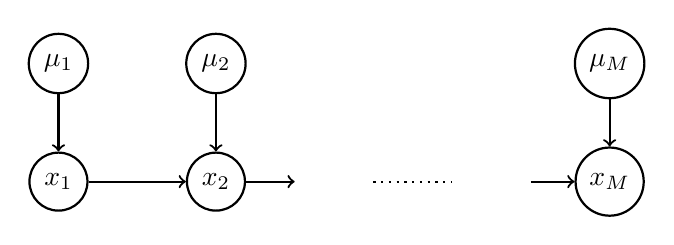
\begin{tikzpicture}
        % First pair
        \node[circle,draw=black,line width=0.8pt,minimum size=0.6cm] (mu1) at (0,1.5) {$\mu_1$};
        \node[circle,draw=black,line width=0.8pt,minimum size=0.6cm] (x1) at (0,0) {$x_1$};
        
        % Second pair
        \node[circle,draw=black,line width=0.8pt,minimum size=0.6cm] (mu2) at (2,1.5) {$\mu_2$};
        \node[circle,draw=black,line width=0.8pt,minimum size=0.6cm] (x2) at (2,0) {$x_2$};
        
        % Last pair
        \node[circle,draw=black,line width=0.8pt,minimum size=0.6cm] (muM) at (7,1.5) {$\mu_M$};
        \node[circle,draw=black,line width=0.8pt,minimum size=0.6cm] (xM) at (7,0) {$x_M$};
        
        % Vertical connections
        \draw[->,black,line width=0.8pt] (mu1) -- (x1);
        \draw[->,black,line width=0.8pt] (mu2) -- (x2);
        \draw[->,black,line width=0.8pt] (muM) -- (xM);
        
        % Horizontal connections with spaced ellipsis
        \draw[->,black,line width=0.8pt] (x1) -- (x2);
        \draw[->,black,line width=0.8pt] (x2) -- (3,0);
        \draw[dotted, black,line width=0.8pt] (4,0) -- (5,0);
        \draw[->,black,line width=0.8pt] (6,0) -- (xM);
      \end{tikzpicture}
      \caption{} 
      \label{fig:dir_prior}
    \end{figure}

    We could also choose to share a common prior over the parameters, trading flexibility for computational feasibility. 

    \begin{figure}[H]
      \centering 
      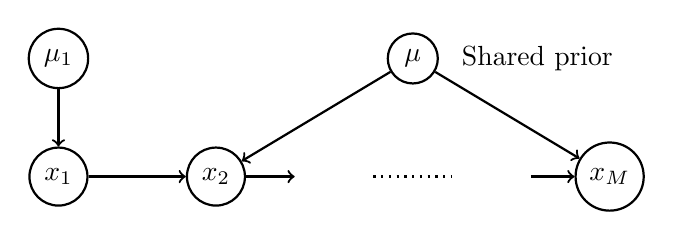
\begin{tikzpicture}
        % First mu node with x1
        \node[circle,draw=black,line width=0.8pt,minimum size=0.6cm] (mu1) at (0,1.5) {$\mu_1$};
        \node[circle,draw=black,line width=0.8pt,minimum size=0.6cm] (x1) at (0,0) {$x_1$};
        
        % Second x node
        \node[circle,draw=black,line width=0.8pt,minimum size=0.6cm] (x2) at (2,0) {$x_2$};
        
        % Last x node
        \node[circle,draw=black,line width=0.8pt,minimum size=0.6cm] (xM) at (7,0) {$x_M$};
        
        % Shared mu node
        \node[circle,draw=black,line width=0.8pt,minimum size=0.6cm] (mu) at (4.5,1.5) {$\mu$};
        
        % Label for shared prior
        \node[right] at (5,1.5) {Shared prior};
        
        % Vertical connections
        \draw[->,black,line width=0.8pt] (mu1) -- (x1);
        \draw[->,black,line width=0.8pt] (mu) -- (x2);
        \draw[->,black,line width=0.8pt] (mu) -- (xM);
        
        % Horizontal connections with spaced ellipsis
        \draw[->,black,line width=0.8pt] (x1) -- (x2);
        \draw[->,black,line width=0.8pt] (x2) -- (3,0);
        \draw[dotted, black,line width=0.8pt] (4,0) -- (5,0);
        \draw[->,black,line width=0.8pt] (6,0) -- (xM);
      \end{tikzpicture}
      \caption{} 
      \label{fig:shared_dir_prior}
    \end{figure}
  \end{example}

  Another way to make more compact representations is through parameterized models. For example, if we have to compute $p(y = 1 \mid \mathbf{x}_1, \ldots, \mathbf{x}_M)$, this in general has $O(K^M)$ parameters. However, we can obtain a more parsimonious form by using a logistic function acting on a linear combination of the parent variables 
  \begin{equation}
    p(y = 1 \mid \mathbf{x}_1, \ldots, \mathbf{x}_m) = \sigma \bigg( w_0 + \sum_{i=1}^M w_i x_i \bigg) = \sigma(\mathbf{w}^T \mathbf{x})
  \end{equation}
  We can look at an example how this is applied to sampling from high-dimensional Gaussian with \textbf{linear Gaussian models}.  


  \begin{example}[Multivariate Gaussian]
    Consider an arbitrary acyclic graph over $D$ random variables, in which eachnode represents a single continuous Gaussian distribution with its mean given by a linear function of its parents. 
    \[p(x_i \mid \mathbf{pa}_i) = N \bigg( x_i \bigg| w_{ij} x_j + b_j, v_i \bigg) \]
    Given a multivariate Gaussian, let us try to decompose it into a directed graph. The log of the joint distribution takes form 
    \[\ln p(\mathbf{x}) = \sum_{i=1}^D \ln p(x_i \mid \mathrm{pa}_i) = - \sum_{i=1}^D \frac{1}{2 v_i} \bigg( x_i - \sum_{j \in \mathrm{pa}_i} w_{ij} x_j - b_i \bigg)^2 + \mathrm{const}\]
    To compute the mean, we can see that by construction, every $x_i$ is dependent on its ancestors, so 
    \[x_i = \sum_{j \in \mathrm{pa}_i} w_{ij} x_j + b_i + \sqrt{v_i} \epsilon_i, \;\; \epsilon_i \sim N(0, 1)\]
    so by linearity of expectation, we have 
    \[\mathbb{E}[x_i] = \sum_{j \in \mathrm{pa}_i} w_{ij} \mathbb{E}[x_j] + b_i\]
    So again, we can start at the top of the graph and compute the expectation. To compute covariance, we can obtain the $i, j$th element of $\boldsymbol{\Sigma}$ with a recurrence relation: 
    \begin{align*} 
      \Sigma_{ij} & = \mathbb{E}[ (x_i - \mathbb{E}[x_i]) (x_j - \mathbb{E}[x_j])] \\
                  & = \mathbb{E} \bigg[ (x_i - \mathbb{E}[x_i]) \bigg( \sum_{k \in \mathrm{pa}_j} w_{j k} (x_k - \mathbb{E}[x_k])  + \sqrt{v_i} \epsilon_j\bigg) \bigg] \\
                  & = \sum_{k \in \mathrm{pa}_j} w_{j k} \Sigma_{ik} + I_{ij} v_j
    \end{align*}
    If there were no links in the graphs, then the $w_{ij}$'s are $0$, and so $\mathbb{E}[\mathbf{x}] = [b_1, \ldots, b_D]$, making the covariance diagonal.If the graph is fully connected, then the total number of parameters is $D + D(D-1)/2$, which corresponds to a general symmetric covariance matrix.  
  \end{example}

  \begin{example}[Bilinear Gaussian Model]
    Consider the following model
    \begin{align*}
      u & \sim N(0, 1) \\
      v & \sim N(0, 1) \\
      r & \sim N(u v, 1)
    \end{align*}
    where the mean of $r$ is a product of $2$ Gaussians. This is also a parameterized model. 

    \begin{figure}[H]
      \centering 
      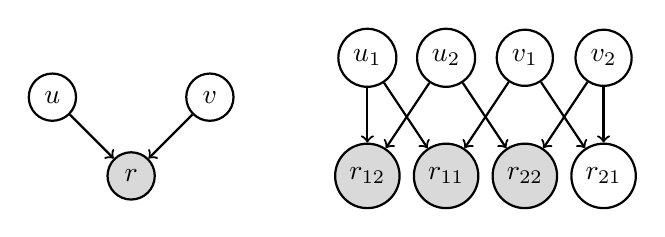
\begin{tikzpicture}
        % Left network
        \node[circle,draw=black,line width=0.8pt,minimum size=0.6cm] (u) at (-2,1) {$u$};
        \node[circle,draw=black,line width=0.8pt,minimum size=0.6cm] (v) at (0,1) {$v$};
        \node[circle,draw=black,line width=0.8pt,fill=gray!30,minimum size=0.6cm] (r) at (-1,0) {$r$};

        % Draw directed edges for left network
        \draw[->,black,line width=0.8pt] (u) -- (r);
        \draw[->,black,line width=0.8pt] (v) -- (r);

        % Right network
        \node[circle,draw=black,line width=0.8pt,minimum size=0.6cm] (u1) at (2,1.5) {$u_1$};
        \node[circle,draw=black,line width=0.8pt,minimum size=0.6cm] (u2) at (3,1.5) {$u_2$};
        \node[circle,draw=black,line width=0.8pt,minimum size=0.6cm] (v1) at (4,1.5) {$v_1$};
        \node[circle,draw=black,line width=0.8pt,minimum size=0.6cm] (v2) at (5,1.5) {$v_2$};
        
        \node[circle,draw=black,line width=0.8pt,fill=gray!30,minimum size=0.6cm] (r12) at (2,0) {$r_{12}$};
        \node[circle,draw=black,line width=0.8pt,fill=gray!30,minimum size=0.6cm] (r11) at (3,0) {$r_{11}$};
        \node[circle,draw=black,line width=0.8pt,fill=gray!30,minimum size=0.6cm] (r22) at (4,0) {$r_{22}$};
        \node[circle,draw=black,line width=0.8pt,minimum size=0.6cm] (r21) at (5,0) {$r_{21}$};

        % Draw directed edges for right network
        \draw[->,black,line width=0.8pt] (u1) -- (r12);
        \draw[->,black,line width=0.8pt] (u1) -- (r11);
        \draw[->,black,line width=0.8pt] (u2) -- (r12);
        \draw[->,black,line width=0.8pt] (u2) -- (r22);
        \draw[->,black,line width=0.8pt] (v1) -- (r11);
        \draw[->,black,line width=0.8pt] (v1) -- (r21);
        \draw[->,black,line width=0.8pt] (v2) -- (r22);
        \draw[->,black,line width=0.8pt] (v2) -- (r21);
      \end{tikzpicture}
      \caption{} 
      \label{fig:bilinear_gaussian}
    \end{figure}
  \end{example}

  \begin{definition}[Conditional Independence in Directed Graphs]
    We say that $a$ is independent of $b$ given $c$ if 
    \[p(a \mid b, c) = p(a \mid c)\]
    or equivalently, 
    \[p(a, b \mid c) = p(a \mid b, c)\, p(b \mid c) = p(a \mid c) \, p(b \mid c)\]
    Conveniently, we can directly read conditional independence properties of the joint distribution from the graph without any analytical measurements. 
  \end{definition}

  \begin{example}[Conditional Independence on Dataset]
    We can demonstrate conditional independence with iid data. Consider the problem of density estimation of some dataset $\mathcal{D} = \{x_i\}$ with some parameterized distribution of $\mu$. Originally, the observations are not independent since they depend on $\mu$. 
    \begin{equation}
      p(\mathcal{D}) = \int_{\mu} p(\mathcal{D} \mid \mu) \, p(\mu)\, d\mu 
    \end{equation}

    \begin{figure}[H]
      \centering 
      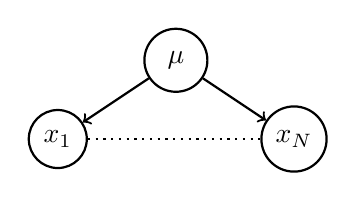
\begin{tikzpicture}
        \node[circle,draw=black,line width=0.8pt,minimum size=0.8cm] (mu2) at (0,-1) {$\mu$};
        
        \node[circle,draw=black,line width=0.8pt,minimum size=0.6cm] (x12) at (-1.5,-2) {$x_1$};
        \node[circle,draw=black,line width=0.8pt,minimum size=0.6cm] (xn2) at (1.5,-2) {$x_N$};
        
        \draw[->,black,line width=0.8pt] (mu2) -- (x12);
        \draw[->,black,line width=0.8pt] (mu2) -- (xn2);
        \draw[dotted,black,line width=0.8pt] (x12) -- (xn2);
      \end{tikzpicture}
      \caption{}
      \label{fig:conditional_indep_iid_1}
    \end{figure}

    If we condition on $\mu$ and considered the joint over the observed variables, the variables are independent. 
    \begin{equation}
      p(\mathcal{D} \mid \mu) = \prod_{n=1}^N p(x_n \mid \mu)
    \end{equation}

    \begin{figure}[H]
      \centering 
      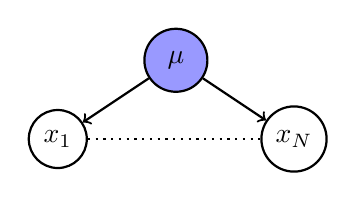
\begin{tikzpicture}
        \node[circle,draw=black,fill=blue!40,line width=0.8pt,minimum size=0.8cm] (mu1) at (0,2) {$\mu$};
        
        \node[circle,draw=black,line width=0.8pt,minimum size=0.6cm] (x11) at (-1.5,1) {$x_1$};
        \node[circle,draw=black,line width=0.8pt,minimum size=0.6cm] (xn1) at (1.5,1) {$x_N$};
        
        \draw[->,black,line width=0.8pt] (mu1) -- (x11);
        \draw[->,black,line width=0.8pt] (mu1) -- (xn1);
        \draw[dotted,black,line width=0.8pt] (x11) -- (xn1);
      \end{tikzpicture}
      \caption{}
      \label{fig:conditional_indep_iid_2}
    \end{figure}    
  \end{example}

  The example above identifies a node (the parent $\mu$) where, if observed, causes the rest of the nodes to become independent. We can extend on this idea by taking an arbitrary $x_i$ and finding a set of nodes such that if they are observed, then $x_i$ is indepedent from every other node. 

  \begin{definition}[Markov Blanket in Directed Graphs]
    The \textbf{Markov blanket} of a node is the minimal set of nodes that must be observed to make this node independent of all other nodes. It turns out that the parents, children, and coparents are all in the Markov blanket. 

    \begin{figure}[H]
      \centering 
      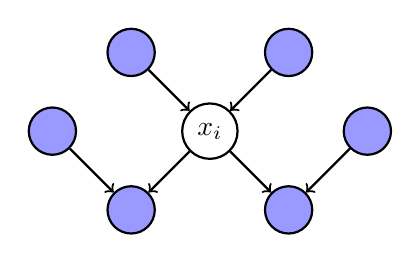
\begin{tikzpicture}
        % Central node
        \node[circle,draw=black,line width=0.8pt,minimum size=0.6cm] (c) at (0,0) {$x_i$};
        
        % Parent nodes (top)
        \node[circle,draw=black,fill=blue!40,line width=0.8pt,minimum size=0.6cm] (p1) at (-1,1) {};
        \node[circle,draw=black,fill=blue!40,line width=0.8pt,minimum size=0.6cm] (p2) at (1,1) {};
        
        % Middle level nodes
        \node[circle,draw=black,fill=blue!40,line width=0.8pt,minimum size=0.6cm] (m1) at (-2,0) {};
        \node[circle,draw=black,fill=blue!40,line width=0.8pt,minimum size=0.6cm] (m2) at (2,0) {};
        
        % Children nodes (bottom)
        \node[circle,draw=black,fill=blue!40,line width=0.8pt,minimum size=0.6cm] (c1) at (-1,-1) {};
        \node[circle,draw=black,fill=blue!40,line width=0.8pt,minimum size=0.6cm] (c2) at (1,-1) {};
        
        \draw[->,black,line width=0.8pt] (p1) -- (c);
        \draw[->,black,line width=0.8pt] (p2) -- (c);
        \draw[->,black,line width=0.8pt] (c) -- (c1);
        \draw[->,black,line width=0.8pt] (c) -- (c2);
        \draw[->,black,line width=0.8pt] (m1) -- (c1);
        \draw[->,black,line width=0.8pt] (m2) -- (c2);
      \end{tikzpicture}
      \caption{} 
      \label{fig:markov_blanket_directed}
    \end{figure} 

    Note that 
    \begin{equation}
      p(x_i \mid x_{j \neq i}) = \frac{p(x_1, \ldots, x_M)}{\int p(x_1, \ldots, x_M) \,dx} = \frac{\prod_k p(x_k \mid \mathrm{pa}_k)}{\int \prod_k p(x_k \mid \mathrm{pa}_k) \,dx_i}
    \end{equation}
  \end{definition} 

  One final interpretation is that we can view directed graphs as \textbf{distribution filters}. We take the joint probability distribution, will starts off as fully connected, and the directed graphs ``filters" away the edges that are not needed. Therefore, the joint probability distribution $p(\mathbf{x})$ is only allows through the filter if and only if it satisfies the factorization property. 

\subsection{Markov Random Field (Undirected Graphical Models)}

  As the name implies, undirected models use undirected graphs, which are used to model relationships that go both ways rather than just one. Unlike directed graphs, which are useful for expressing casual relationships between random variables, undirected graphs are useful for expressing soft constraints between random variables.  

  \begin{definition}[Conditional Independence in Undirected Graphs]
    Fortunately, conditional independence is easier compared to directed models. We can say $A$ is conditionally independent to $B$ given $C$ if $C$ blocks all paths between any node in $A$ and any node in $B$. 

    \begin{figure}[H]
      \centering 
      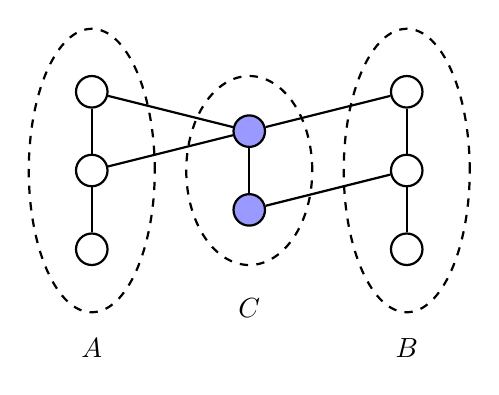
\begin{tikzpicture}
        \node[circle,draw=black,line width=0.8pt,minimum size=0.4cm] (a1) at (-2,1) {};
        \node[circle,draw=black,line width=0.8pt,minimum size=0.4cm] (a2) at (-2,0) {};
        \node[circle,draw=black,line width=0.8pt,minimum size=0.4cm] (a3) at (-2,-1) {};

        \node[circle,draw=black,line width=0.8pt,fill=blue!40,minimum size=0.4cm] (c1) at (0,0.5) {};
        \node[circle,draw=black,line width=0.8pt,fill=blue!40,minimum size=0.4cm] (c2) at (0,-0.5) {};

        % Right cluster (B)
        \node[circle,draw=black,line width=0.8pt,minimum size=0.4cm] (b1) at (2,1) {};
        \node[circle,draw=black,line width=0.8pt,minimum size=0.4cm] (b2) at (2,0) {};
        \node[circle,draw=black,line width=0.8pt,minimum size=0.4cm] (b3) at (2,-1) {};

        % Draw edges
        \draw[black,line width=0.8pt] (a1) -- (a2);
        \draw[black,line width=0.8pt] (a2) -- (a3);
        \draw[black,line width=0.8pt] (a1) -- (c1);
        \draw[black,line width=0.8pt] (a2) -- (c1);
        \draw[black,line width=0.8pt] (c1) -- (c2);
        \draw[black,line width=0.8pt] (c1) -- (b1);
        \draw[black,line width=0.8pt] (c2) -- (b2);
        \draw[black,line width=0.8pt] (b1) -- (b2);
        \draw[black,line width=0.8pt] (b2) -- (b3);

        % Draw dashed ellipses around clusters
        \draw[color={black},dashed,line width=0.8pt] (-2,0.0) ellipse (0.8cm and 1.8cm) node[below=2cm] {$A$};
        \draw[color={black},dashed,line width=0.8pt] (0,0) ellipse (0.8cm and 1.2cm) node[below=1.5cm] {$C$};
        \draw[color={black},dashed,line width=0.8pt] (2,0.0) ellipse (0.8cm and 1.8cm) node[below=2cm] {$B$};
      \end{tikzpicture}
      \caption{$A$ is conditionally independent given $C$, denoted $A \perp\!\!\!\perp B|C$. } 
      \label{fig:undirected_conditional_independence}
    \end{figure}
  \end{definition}

  \begin{definition}[Markov Blanket in Undirected Graphs]
    The Markov blanket of a node, which is the minimal set of nodes that must be observered to make this node independent of the rest of the nodes, is simply the nodes that are directly connected to that node. 

    \begin{figure}[H]
      \centering 
      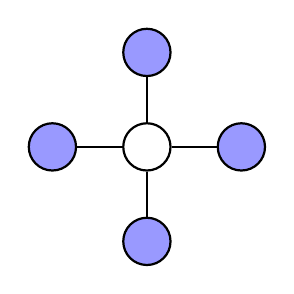
\begin{tikzpicture}
        % Central node
        \node[circle,draw=black,line width=0.8pt,minimum size=0.6cm] (c) at (0,0) {};
        
        % Filled outer nodes
        \node[circle,draw=black,fill=blue!40,line width=0.8pt,minimum size=0.6cm] (n1) at (0,1.2) {};
        \node[circle,draw=black,fill=blue!40,line width=0.8pt,minimum size=0.6cm] (n2) at (1.2,0) {};
        \node[circle,draw=black,fill=blue!40,line width=0.8pt,minimum size=0.6cm] (n3) at (0,-1.2) {};
        \node[circle,draw=black,fill=blue!40,line width=0.8pt,minimum size=0.6cm] (n4) at (-1.2,0) {};
        
        % Draw edges
        \draw[black,line width=0.8pt] (c) -- (n1);
        \draw[black,line width=0.8pt] (c) -- (n2);
        \draw[black,line width=0.8pt] (c) -- (n3);
        \draw[black,line width=0.8pt] (c) -- (n4);
      \end{tikzpicture}
      \caption{Once the neighbors of a node are realized, the node is independent of the rest of the nodes. } 
      \label{fig:markov_blanket_undirected}
    \end{figure}

    Therefore, the conditional distribution of $x_i$ conditioned on all the variables in the graph is dependent only on the variables in the Markov blanket. 
  \end{definition}

  Now, let us talk about how we can actually define a probability distribution with this graph. 

  \begin{definition}[Clique] 
    In an undirected graph, a \textbf{clique} is a set of nodes such that there exists a link between all pairs of nodes in that subset. A \textbf{maximal clique} is a clique such that it is not possible to include any other nodes in the set without it ceasing it to be a clique. 
  \end{definition}

  Given a joint random variable $\mathbf{x}$  represented by an undirected graph, the joint distribution is given by the product of non-negative potential functions over the maximal cliques 
  \begin{equation}
    p(\mathbf{x}) = \frac{1}{Z} \prod_C \phi_C (x_C)
  \end{equation}
  where 
  \begin{equation}
    Z = \int p(\mathbf{x}) \,d\mathbf{x}
  \end{equation}
  is the normalizing constant, called the \textbf{partition function}. That is, each $x_C$ is a maximal clique and $\phi_C$ is the nonnegative potential function of that clique. 

  This assignment looks pretty arbitrary. How do we know that any arbitrary joint distribution of $\mathbf{x}$, which has a undirected graphical representation, can be represented as the product of a bunch of functions over the maximum cliques? Fortunately, there is a mathematical result that proves this. 

  \begin{theorem}[Hammersley-Clifford] 
    The joint probability distribution of any undirected graph can be written as the product of potential functions on the maximal cliques of the graph. Furthermore, for any factorization of these potential functions, there exists an undirected graph for which is the joint.  
  \end{theorem} 


  \begin{example}
    For example, the joint distribution of the graph below
    \begin{figure}[H]
      \centering 
      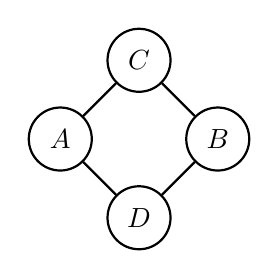
\begin{tikzpicture}
        % Define nodes
        \node[circle,draw=black,line width=0.8pt,minimum size=0.8cm] (A) at (-1,0) {$A$};
        \node[circle,draw=black,line width=0.8pt,minimum size=0.8cm] (B) at (1,0) {$B$};
        \node[circle,draw=black,line width=0.8pt,minimum size=0.8cm] (C) at (0,1) {$C$};
        \node[circle,draw=black,line width=0.8pt,minimum size=0.8cm] (D) at (0,-1) {$D$};

        % Draw thick edges
        \draw[black,line width=0.8pt] (A) -- (C);
        \draw[black,line width=0.8pt] (A) -- (D);
        \draw[black,line width=0.8pt] (B) -- (C);
        \draw[black,line width=0.8pt] (B) -- (D);
      \end{tikzpicture}
      \caption{} 
      \label{fig:hammersley_clifford_ex}
    \end{figure}
    factorizes into 
    \begin{equation}
      p(A, B, C, D) = \frac{1}{Z} \phi(A, C) \, \phi(C, B) \, \phi(B, D) \, \phi(A, D)
    \end{equation}
  \end{example}

  Note that each potential function $\phi$ is a mapping from the joint configuration of random variables in a clique to non-negative real numbers. The choice of potential functions is not restricted to having specific probabilistic interpretations, but since they must be nonnegative, we can just represent them as an exponential. The negative sign is not needed, but is a remnant of physics notation. 
  \begin{equation}
    p (\mathbf{x}) = \frac{1}{Z} \prod_C \phi_C (x_C) = \frac{1}{Z} \exp \bigg\{ - \sum_C E(x_C) \bigg\} = \frac{1}{Z} \underbrace{\exp \big\{ - E(\mathbf{x}) \big\}}_{\substack{\text{Boltzmann}\\ \text{distribution}}}
  \end{equation}

  Any distribution that can be represented as the form above is called a \textbf{Boltzmann distribution}. So far, all we stated is that the joint probability distribution can be expressed as the product of a bunch of potential functions, but besides the fact that it is nonnegative, there is no probabilistic interpretation of these potentials (or equivalently, the energy functions). While this does give us greater flexibility in choosing potential functions, we must be careful in choosing them (e.g. choosing something like $x^2$ may cause the integral to diverge, making the joint not well-defined).

  Clearly, these potential functions over the cliques should express which configuration of the local variables are preferred to others. It should assign higher values to configurations that are deemed (either by assumption or through training data) to be more probable. That is, each potential is like an ``expert" that provides some opinion (the value) on a configuration, and the product of the values of all the potential represents the total opinion of all the experts. Therefore, global configurations with relatively high probabilities are those that find a good balance in satisfying the (possibly conflicting) influences of the clique potentials. 

  \begin{example}[Transmission of Colds] 
    Say that you want to model a distribution over three binary variables: whether you or not you, your coworker, and your roommate is sick ($0$ represents sick and $1$ represents healthy). Then, you can make simplifying assumptions that your roommate and your coworker do not know each other, so it is very unlikely that one of thme will give the other an infection such as a cold directly. Therefore, we can model the indirect transmission of a cold from your coworker to your roommate by modeling the transmission of the cold from your coworker to you and then you to your roommate. Therefore, we have a model of form

    \begin{center}
      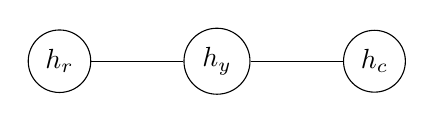
\begin{tikzpicture}
        \node[circle,draw] (hr) at (0,0) {$h_r$};
        \node[circle,draw] (hy) at (2,0) {$h_y$};
        \node[circle,draw] (hc) at (4,0) {$h_c$};

        \draw (hr) -- (hy);
        \draw (hy) -- (hc);
      \end{tikzpicture}
    \end{center}
    One max clique contains $h_y$ and $h_c$. The factor for this clique can be defined by a table and might have values resembling these. 

    \begin{table}[H]
      \centering
      \begin{tabular}{c|c|c|}
      \cline{2-3}
      & \( h_y = 0 \) & \( h_y = 1 \) \\ \hline
      \multicolumn{1}{|c|}{\( h_c = 0 \)} & 2 & 1 \\ \hline
      \multicolumn{1}{|c|}{\( h_c = 1 \)} & 1 & 10 \\ \hline
      \end{tabular}
      \caption{States and Values of \( h_y \) and \( h_c \)}
    \end{table}

    This table completely describes the potential function of this clique. Both of you are usually healthy, so the state $(1, 1)$ gets the maximum value of $1$. If one of you are sick, then it is likely that the other is sick as well, so we have a value of $2$ for $(0, 0)$. Finally, it is most unlikely that one of you is sick and the other healthy, which has a value of $1$. 
  \end{example}

\subsection{Hidden Markov Models}

\subsection{Expectation-Maximization Algorithm} 

  EM algorithm is used to optimize latent variable models. Recall \textbf{Jensen's Inequality}: Given a convex function $f: \mathbb{R} \longrightarrow \mathbb{R}$ (meaning that $f^{\prime\prime} (x) \geq 0$ for all $x$) and a random variable $X$, we have 
  \[\mathbb{E}\big(f(X)\big) \geq f\big(\mathbb{E}(X)\big) \]
  Moreover, if $f$ is strictly convex, then $\mathbb{E}\big( f(X)\big) = f\big(\mathbb{E}(X)\big)$ holds true if and only if $X = \mathbb{E}(X)$ with probability $1$ (i.e. if $X$ is a constant). 

  Suppose we have an estimation problem given the training set $\{x^{(i)}\}_{i=1}^n$. We have latent variable model $p(x, z; \theta)$ with $z$ being the latent variable of discrete, finite random variable $Z$, with density $p_Z (z)$. Let us denote the density of $X$ as $p_X$. Then, the random variable $X$ can be interpreted as us first generating $z$ from $Z$, and then computing $X\,|\,Z = z$.  
  \[\text{Compute } X = \text{Compute } Z \text{ and then } \begin{cases} 
  \text{Compute } X \,|\, Z = 1 \\
  \text{Compute } X \,|\, Z = 2 \\
  \ldots \\
  \text{Compute } X \,|\, Z = k
  \end{cases}\]

  Let us clarify some notation: 
  \begin{itemize}
    \item The distribution that we will iteratively reassign over and over again is $Z$, with density $p_Z$ that maps $z \mapsto \phi_z$, where $\phi$ is a vector that represents the density.
    \item The $k$ conditional (not necessarily Gaussian) distributions that we will iteratively reassign over and over again is $X_1, X_2, \ldots, X_k$, with densities $p_{X_1} (x), \ldots, p_{X_k} (x)$ that maps $x \mapsto p_{X_j} (x)$.
    \item The distribution of the entire random variable $X$ will have density $p_X (x)$. Since we are iteratively reassigning the densities $p_Z$ and $p_{X_j}$, this joint distribution of $X$ will also get modified.
  \end{itemize}

  The EM algorithm in the general case has the following steps: 
  \begin{enumerate}
    \item We initialize the value of $\theta$ in some way. Note that within this $\theta$ are the parametizations of the initial multinomial density $p_Z$, which is our initial "guess" of the distribution of $Z$.
    \item \textbf{(E Step)} The log likelihood of the given data $\{ x^{(i)}\}_{i=1}^n$ with respect to the parameter $\theta$ (which encodes all parameters of distribution $Z$ and all $X\,|\,Z$) is 
      \[l(\theta) = \sum_{i=1}^n \log\, p_X \big( x^{(i)}; \, \theta \big)\]
    It turns out that explicitly finding the maximum likelihood estimates of the parameters $\theta$ is hard because it results in a difficult, non-convex optimization problem. So, we tackle this another way. 
    
    To start, we can see that the summation isn't too crucial, so we can focus on minimizing each $\log \, p_X \big(x^{(i)}; \, \theta \big)$ and summing in the end. We can calculate this by conditioning over all $j = 1, \ldots, k$ generated from $Z$ (which we have guessed to have an initial density of $p_Z$). That is, we must find for each $i = 1, 2, \ldots, n$ 
    \begin{align*} 
      \max_\theta \log \, p_X \big( x^{(i)}; \, \theta \big) & = \max_\theta \log \, \bigg(\sum_{j=1}^k p_X \big(x^{(i)}, Z = j; \, \theta\big) \bigg) \\
      & = \max_\theta \log \bigg( \sum_{j=1}^k p_X \big( x^{(i)}\,|\, Z = j; \, \theta\big) p_Z \big( j; \, \theta \big) \bigg) \\
      & = \max_\theta \log \bigg( \sum_{j=1}^k p_{X_j} \big( x^{(i)} ;\, \theta\big) p_Z \big( j; \, \theta \big) \bigg)
    \end{align*}
    To find this maximum value, we can focus on the first equality and see that by Jensen's inequality (with conCAVE, not convex, $f(x) = \log x$ over domain $x \in \mathbb{R}^+$), the following holds true for all $\theta$ and more importantly, for \textit{any arbitrary density function} $p_Z^{*i}$.  
    \begin{align*} 
      \log p_X \big(x^{(i)};\, \theta\big) & = \log \bigg( \sum_{j=1}^k p_X \big(x^{(i)}, Z = j;\, \theta \big) \bigg) \\ 
      & = \log \bigg( \sum_{j=1}^k p_Z^{*i} \big(j \big)\, \frac{p_X \big(x^{(i)}, Z = j;\, \theta \big)}{p_Z^{*i} \big(j \big)} \bigg) \\
      & = \log \Bigg(\mathbb{E}_{j \sim p_Z^{*i}} \bigg( \frac{p(x^{(i)}, Z = j; \, \theta)}{p_Z^{*i} \big(j \big)}\bigg)\Bigg) \\
      & \geq \mathbb{E}_{j \sim p_Z^{*i}} \Bigg( \log \bigg( \frac{p(x^{(i)}, Z = j; \, \theta)}{p_Z^{*i} \big(j \big)} \bigg) \Bigg) \\
      & = \sum_{j=1}^k p_Z^{*i} (j) \, \log\bigg( \frac{p(x^{(i)}, Z = j; \, \theta)}{p_Z^{*i} (j)} \bigg) = \text{ELBO} \big( x^{(i)}; \,p_Z^{*i}, \theta \big)
    \end{align*}
    The final term, called the \textbf{evidence lower bound} (ELBO), is just the expectation of $\log \frac{p(x^{(i)}, Z = j; \, \theta)}{p_Z^{*i} (j)}$ with respect to $j$ drawn from density $p_Z^{*i}$, which is denoted with $\mathbb{E}_{j \sim p_Z^{*i}}$. 
    
    Summing over all $n$ examples, we have a lower bound for the entire log likelihood for \textit{any} set of density functions $p_Z^{*1}, p_Z^{*2}, \ldots, p_Z^{*n}$: 
    \begin{align*} 
      l(\theta) = \sum_{i=1}^n \log p(x^{(i)}; \, \theta) & \geq \sum_{i=1}^n \text{ELBO}(x^{(i)}; \, p_Z^{*i}, \theta) \\
      & = \sum_{i=1}^n \sum_{j=1}^k p_Z^{*i} (j) \, \log\bigg( \frac{p(x^{(i)}, Z = j; \, \theta)}{p_Z^{*i} (j)} \bigg)
    \end{align*}
    Our job now is to choose the correct density functions $p_Z^{*i}$'s such that the lower bound is maximized. It turns out that we can do even better: equality is satisfied if and only if we set 
    \begin{align*} 
      p_Z^{*i} (j) & \equiv p_Z \big( j\,|\, x^{(i)}; \, \theta \big) \\
      & \equiv p_Z^{(i)} \big( j; \, \theta \big) \text{ for all } i = 1, 2, \ldots, n
    \end{align*}
    which is simply the posterior distribution of the multinomial given the observed sample $x^{(i)}$, which we can easily calculate using Bayes' rule. Substituting this into $p_Z^{*i}$ leads to the equality 
    \begin{align*} 
      l(\theta) = \sum_{i=1}^n \log p (x^{(i)}; \, \theta) 
      & = \sum_{i=1}^n \text{ELBO}\big(x^{(i)}; p_Z^{(i)}, \, \theta \big) \\
      & = \sum_{i=1}^n \sum_{j=1}^k p_Z^{(i)} \big( j; \, \theta \big) \, \log\bigg( \frac{p(x^{(i)}, Z = j; \, \theta)}{p_Z^{(i)} \big( j; \, \theta \big)} \bigg) \\
      & = \sum_{i=1}^n \sum_{j=1}^k p_Z \big( j\,|\, x^{(i)}; \, \theta \big) \, \log\bigg( \frac{p(x^{(i)}, Z = j; \, \theta)}{p_Z \big( j\,|\, x^{(i)}; \, \theta \big)} \bigg)
    \end{align*}
    In summary, this E step has taken the log-likelihood function $l(\theta)$ (representing (the log of) the probability of all the $x^{(i)}$'s landing where they are given the parameters $\theta$), which is abstract and hard-to-optimize, and converted it into an equivalent form as the sum of a bunch of ELBO functions optimized with the density parameters begin assigned $p_Z^{*i} = p_Z^{(i)}$. 
    
    But remember that these optimal densities $p_Z^{*i} = p_Z^{(i)}$ make the right and left hand side equivalent only for a \textbf{fixed value} of $\theta$! So, the right hand side is only equivalent to $l(\theta)$ only for that one value of $\theta$, but as soon as we set $\theta$ to something else, the right hand side evaluated with $p_Z^{*i} = p_Z^{(i)}$ are not equal.
    \item \textbf{(M Step)} Since we have found some equivalent form of $l(\theta)$ for the fixed $\theta$ that was initialized, we can now just maximize the right hand side with respect to $\theta$, while fixing the $p_Z^{*i} = p_Z^{(i)}$'s. Therefore, we find and set the value of $\theta$ as 
    \begin{align*}  
      \theta & = \text{arg}\; \max_\theta \sum_{i=1}^n \text{ELBO} \big( x^{(i)}; \, p_Z^{(i)}, \theta \big) \\
      & = \text{arg}\; \max_\theta \sum_{i=1}^n \sum_{j=1}^k p_Z^{(i)} (j)\; \log \bigg( \frac{p(x^{(i)}, Z = j; \, \theta)}{p_Z^{(i)} (j)} \bigg) \\
      & = \text{arg}\; \max_\theta \sum_{i=1}^n \sum_{j = 1}^k p_Z \big(j\,|\, x^{(i)}; \, \theta \big)\, \log \bigg( \frac{p(x^{(i)}, Z = j; \, \theta)}{p_Z \big(j\,|\, x^{(i)}; \, \theta \big)} \bigg)
    \end{align*}
    In the case where the parameter $\theta$ consist of $\phi, \mu_1, \ldots, \mu_k, \Sigma_1, \ldots, \Sigma_k$ like in the GMM model, it happens so that the maximum is found by computing $\phi$ to be the average of the $\phi^{(i)}$'s, each $\mu_j$ to be the weighed averages of the points, and each $\Sigma_j$ as the equation above. For other distributions, the formula for the maximum must be mathematically found (or algorithmically computed) with respect to parameter $\theta$.
    \item We have now reassigned the entire value of $\theta$, meaning that the parameters representing our guess of density $p_Z$ of $Z$ has also been modified. With this new value of $\theta$, we repeat steps 2 and 3 until convergence.
  \end{enumerate}

  For some intuition, we can visualize $l$ as a function of $\theta$. For the sake of visuals, we will assume that $\theta \in \mathbb{R}$ and $l: \mathbb{R} \longrightarrow \mathbb{R}$. On the contrary to what a visual is supposed to do, we want to point out that we cannot just visualize $l$ as a curve in $\mathbb{R} \times \mathbb{R}$. This can be misleading since then it implies that the optimal $\theta$ value is easy to find, as shown in the left. Rather, we have no clue what the whole curve of $l$ looks like, but we can get little snippets (right). 

  \begin{figure}[H]
    \centering 
    \includegraphics[width=0.6\textwidth]{img/visual_of_l.jpg}
    \caption{} 
    \label{fig:visual_of_l}
  \end{figure}

  Rather, all we can do is hope to take whatever easier-to-visualize, lower-bound functions and maximize them as much as we can in hopes of converging onto $l$. Let us walk through the first two iterations of the EM algorithm. We first initialize $\theta$ to, say $\theta_0$. This immediately induces the lower-bound ELBO-sum function $\sum_{i} \text{ELBO} (x^{(i)};\, p_Z^{*i}, \theta)$, which takes in multinomial density functions $p_Z^{*i} = p_1, p_2, \ldots$ and outputs different functions of $\theta$ that are valid lower bounds. Two of these possible lower-bound functions are shown (in green) for when we input some arbitrary density $p_1, p_2$. However, there exists a density $p_Z^{(i)}$ that produces not only the maximum possible lower-bound (called max ELBO, shown in red) but is equal to $l(\theta)$ for that density input $p_Z^{(i)}$. We maximize this function with respect to $\theta$ to get $\theta_1$ as our next assignment of $\theta$. 

  \begin{figure}[H]
    \centering 
    \includegraphics[width=0.7\textwidth]{img/EM_first_iteration.jpg}
    \caption{} 
    \label{fig:EM_first_iteration}
  \end{figure}

  The next step is identical. Now that we have a new value of $\theta = \theta_1$, this induces the lower-bound ELBO-sum function $\sum_{i} \text{ELBO} (x^{(i)};\, p_Z^{*i}, \theta)$ that also takes in multinomial densities $p_Z^{*i}$ and outputs different functions of $\theta$ that are valid lower-bounds. Two possible lower bounds are shown (in green), but the maximum lower-bound (in blue) is produced when we input density $p_Z^{(i)}$. Since this max ELBO function is equal to $\theta$ for this fixed density input $p_Z^{(i)}$, we maximize this function with respect to $\theta$ to get $\theta_2$ as our next assignment of $\theta$. 

  \begin{figure}[H]
    \centering 
    \includegraphics[width=0.7\textwidth]{img/EM_second_iteration.jpg}
    \caption{} 
    \label{fig:EM_second_iteration}
  \end{figure}

  \begin{definition}[EM Algorithm for General Estimation Problems]
    Given a training set $\{x^{(i)}\}_{i=1}^n \in \mathbb{R}^d$, let us assume that the random variable $X$ that these examples follow can be modeled by specifying a joint distribution of a multinomial and some arbitrary distributions. Let there be $k$ clusters, and let 
    \begin{itemize}
      \item $Z$ be the multinomial distribution representing which Gaussian cluster each example $x$ falls in, with density $p_Z (j)$ and represented by vector $\phi \in \mathbb{R}^k$ so that $\mathbb{P}(Z = j) = \phi_j$. Let the parameters of $\phi$ be encoded in $\theta$.
      \item The set of conditional distributions
        \[X\,|\,Z = j \sim X_j \text{ for } j = 1, 2, \ldots, k\]
      are arbitrary distributions with some parameters, also all encoded in $\theta$.  
    \end{itemize}

    The EM algorithm is described as such: 
    \begin{enumerate}
      \item Initialize $\theta$.
      \item \textbf{(E Step)} Since $l(\theta)$ is bounded below for all $p_Z^{*1}, \ldots, p_Z^{*n}$ as 
        \[l(\theta) \equiv \sum_{i=1}^n \log p\big( x^{(i)}; \, \theta\big) \geq \sum_{i=1}^n \text{ELBO}\big( x^{(i)}; \, p_Z^{*i}, \theta\big)\]
      setting $p_Z^{*i} (j) = p_Z^{(i)} (j) = p_Z \big(j\,|\, x^{(i)}; \, \theta\big)$ for all $i = 1, \ldots, n$ would put $l$ into a new form for these specific fixed values of $p_Z^{*i}$. 
        \[l(\theta) = \sum_{i=1}^n \text{ELBO}\big(x^{(i)}; p_Z^{(i)}, \theta \big)\]
      \item \textbf{(M Step)} We maximize this equivalent form of $l(\theta)$ with respect to $\theta$ whilst fixing the choice of $p_Z^{(i)}$. That is, we set the value of $\theta$ as 
      \begin{align*}  
        \theta & = \text{arg}\; \max_\theta \sum_{i=1}^n \text{ELBO} \big( x^{(i)}; \, p_Z^{(i)}, \theta \big) \\
        & = \text{arg}\; \max_\theta \sum_{i=1}^n \sum_{j=1}^k p_Z^{(i)} (j)\; \log \bigg( \frac{p(x^{(i)}, Z = j; \, \theta)}{p_Z^{(i)} (j)} \bigg) \\
        & = \text{arg}\; \max_\theta \sum_{i=1}^n \sum_{j = 1}^k p_Z \big(j\,|\, x^{(i)}; \, \theta \big)\, \log \bigg( \frac{p(x^{(i)}, Z = j; \, \theta)}{p_Z \big(j\,|\, x^{(i)}; \, \theta \big)} \bigg)
      \end{align*}
      \item We have successfully updated $\theta$. Now, we repeat steps 2 and 3 until convergence. Step 2 can bring improvements because we have changed the $\theta$, which means that there is a new sum of ELBO functions of the $\theta$ that serves as a new lower bound.
    \end{enumerate}
  \end{definition}


